\cleardoublepage

\addcontentsline{toc}{chapter}{\numberline{}3eme chapiter}
\addtocontents{lof}{\textbf{Chapter A3}}

\setcounter{chapter}{3}
\setcounter{section}{0}
\setcounter{figure}{0}

\begin{center}
	\Huge\textbf{3eme chapter}
\end{center}

\section{Introduction}
L’optimisation combinatoire occupe une place très importante dans divers domaines. En effet, elle définit un cadre formel pour de nombreux problèmes dans plusieurs secteurs tels que l’industrie, la finance ou tout simplement les problèmes de la vie quotidienne.
La solution optimale à un problème d’optimisation ne peut que très rarement être déterminée en un temps polynomial. Il est donc souvent nécessaire de trouver des modes de résolution qui fournissent une solution de bonne qualité dans un laps de temps raisonnable. Il existe donc des méthodes de résolution exactes qui sont caractérisées par le fait qu’elles permettent d’obtenir une ou plusieurs solutions optimales, ainsi que des méthodes de résolution approchées qui fournissent des solutions de bonne qualité (proches de l’optimal mais sans garantie d’optimalité) et dont le temps de résolution sera plus faible \cite{zidi2006systeme}.

Ce chapitre sera structuré comme suit : d’abord, nous allons présenter brièvement les techniques de routage dans les RCSFs, par la suite nous nous pencherons sur les techniques d’optimisation combinatoire, exactes et approchées surtout, pour la résolution des problèmes NP-Difficiles. Tout ceci sera clôturé par une conclusion.\\
Depuis une vingtaine d’années, les heuristiques les plus populaires, et également les plus efficaces, sont des techniques générales, appelées méta-heuristiques, qu’il s’agit de l’adapter à chaque problème dont sa complexité est NP-hard. Dans ce chapitre, nous allons définir c’est quoi une méta-heuristique, la classification des méthodes utilisées dans les méta-heuristiques. 

\section{Techniques d’optimisation combinatoire:}
L’importance de l’optimisation combinatoire se justifie d’un coté par la grande difficulté des problèmes d’optimisation et d’un autre coté par la quantité innombrable d’applications pratiques pouvant être formulées sous la forme de tels problèmes. En effet, ces derniers sont souvent faciles à formaliser ou à exprimer, mais peuvent toutefois, être très difficiles à résoudre. Néanmoins, la plupart d’entre eux ne possèdent pas à ce jour de solution efficace valable pour toutes les données. \cite{hao1999metaheuristiques}

Un problème d’optimisation combinatoire est exprimé sous forme d’une fonction objectif ; qui est à maximiser, ou à minimiser, selon le type de problème traité. La résolution d’un tel problème revient à chercher la meilleure solution (optimum global) dans l’ensemble des solutions réalisables, sans pour autant être coincé dans des solutions intermédiaires (optimum locaux), propres à un sous-espace de recherche (voir Figure 3.1).

\begin{figure}[h]
	\centering
	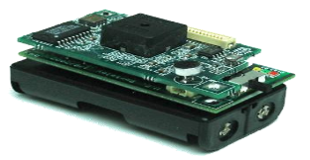
\includegraphics[width=7cm,height=3.7cm]{Chap1/1.png}
	\caption{Différence entre un optimum global et des optima locaux}
	\label{fig:CSF}
\end{figure}

L’élégance des problèmes d’optimisation combinatoire réside dans la possibilité de les modéliser en problèmes de la théorie des graphes et ainsi profiter des outils de cette dernière.

\begin{figure}[h]
	\centering
	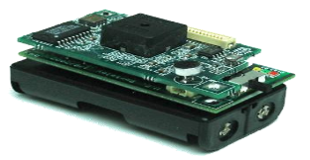
\includegraphics[width=7cm,height=3.7cm]{Chap1/1.png}
	\caption{Différence entre un optimum global et des optima locaux}
	\label{fig:CSF}
\end{figure}

De nombreuses méthodes de résolution ont été développées par la communauté scientifique (recherche opérationnelle, intelligence artificielle).

Ces méthodes sont divisées en deux grandes catégories : les méthodes exactes basées sur l’énumération de toutes les solutions réalisables, chose qui garantie la complétude de la résolution, et les méthodes approchées qui perdent en exactitude pour gagner en efficacité \cite{park2007dominating} . La figure 3.2 illustre un schéma résumant la classification des différentes méthodes discutées le long du chapitre.

\subsection{Méthodes exacte}
Ces méthodes sont dites complètes ou exactes car elles permettent de trouver la solution optimale pour une instance de taille finie dans un temps limité et de prouver son optimalité \cite{puchinger2005combining} . Ces méthodes se basent généralement sur sur une recherche complètes de l’espace des combinaisons afin de trouver une solution optimale. Les algorithmes exacts les plus réussis dans la littérature: 


\begin{enumerate}[label=\alph*)]
	\item \textbf{La méthode séparation et évaluation (Branch and Bound):} elle repose sur une méthode arborescente de recherche d’une solution optimale par séparations et évaluations. Le branch-and-bound est basé sur trois axes principaux: L’évaluation, la séparation, la stratégie de parcours.
	\begin{itemize}
		\item \textbf{L’évaluation: } permet de réduire l’espace de recherche en éliminant quelques sous ensembles qui ne contiennent pas la solution optimale.
		\item \textbf{La séparation: } a pour but de choisir un sous-problème parmi tous ceux non encore choisis. Elle associe donc à chacun une évaluation (valeur minimale) de toutes les solutions le constituant. Un sous-problème peut être supprimé dans le cas où son évaluation est supérieure à la meilleure solution connue.
		\item \textbf{La stratégie de parcours: } c’est le processus qui permet de parcourir l’ensemble des sommets et de déterminer lequel sera séparé.
	\end{itemize}
	\item \textbf{Les méthodes de coupes planes (Cutting-Plane): }type de problème à résoudre. Néanmoins, ce sont des méthodes destinées à trouver des solutions entières pour des problèmes d’optimisation combinatoire qui sont représentés sous forme d’un programme linéaire \cite{schrijver1986theory} .
	\item \textbf{La méthode (Branch and Cut): }face aux problèmes difficiles. De même que l’algorithme du "Branch and Bound". Pour cela la méthode "Branch and Cut" qui conjugue l’effort des deux algorithmes précédemment cités est utilisée \cite{padberg1991branch,padberg1987optimization} .
\end{enumerate}

\subsection{Les méthodes approchées:}
Ces méthodes s’appliquent sur tous les problèmes peut importe leurs complexités et vise à trouver une solution admissible en un temps raisonnable, mais ne garantissent pas  l’optimalité d’un solution. En outre, elles ont démontré leurs robustesses et efficacités face à plusieurs problèmes d’optimisation combinatoires. Elles englobent deux classes : Heuristiques et Méta- heuristiques:
\subsubsection{Heuristiques:}
Les heuristiques sont des règles empiriques simples basées sur l'expérience, ne fournissant pas nécessairement une solution optimale. L’avantage d’utiliser une heuristique réside dans l’efficacité de calculer une solution approchée dans un temps raisonnable et ainsi accélérer le processus de résolution exact, qui peut s’avérer long pour des problèmes à large échelle. Généralement, une heuristique n’offre aucune garantie quant à la qualité de la solution. On peut distinguer une classe d’heuristique qui est les méthodes constructives.

	Les approches constructives construisent une ou plusieurs combinaisons de façon incrémentale, c’est-à-dire, en partant d’une solution initiale vide, et à chaque itération, une variable est choisie (selon une heuristique ou aléatoirement) jusqu’à l’obtention d’une combinaison complète. c'est pour cela ces approches sont dites “basées sur les modèles” dans \cite{zlochin2004model} .\\
Il existe différentes stratégies pour choisir les composants à ajouter à chaque itération, les plus connues étant les stratégies gloutonnes. Ces stratégies consistent à construire une solution pas à pas
sans retour arrière, en prenant à chaque étape la solution qui semble la meilleure localement (selon une heuristique), en espérant obtenir une solution optimale. 

\subsubsection{Meta-Heuristiques:}
Une Méta-heuristique peut être définie comme une méthode algorithmique capable de guider et d’orienter le processus de recherche dans un espace de solution (souvent très grand) à des régions riches en solutions optimales dans le but de trouver des solutions, peut-être pas toujours optimales, en tout cas très proches de l’optimum, en un temps raisonnable.

\subsubsection{Méthodes de voisinage (A solution unique):}
Les méthodes de voisinage se basent sur la notion de voisinage. Elle a plusieurs méthodes chacune débute avec une configuration initiale, et réalise ensuite un processus itératif qui consiste à remplacer la configuration courante par l'un de ses voisins en tenant compte de la fonction de coût. Ce processus s'arrête et retourne la meilleure configuration trouvée quand la condition d'arrêt est réalisée. Cette condition d'arrêt concerne généralement une limite pour le nombre d'itérations, le temps d’exécution ou un objectif à réaliser. Présentant quelques méthodes:

\begin{enumerate}[label=\alph*)]
	\item \textbf{Recuit simulé: } La recherche recuit simulé a été introduite en 1983 par Kirkpatrick et al.[24]. Cette méthode originale est basée sur les travaux bien antérieurs de Metropolis et al. \cite{metropolis1953equation} et elle est considérée comme la plus ancienne méta-heuristique.\\
Le principe de fonctionnement s’inspire d’un processus d’amélioration de la qualité d’un métal solide par recherche d’un état d’énergie minimum correspondant à une structure stable de ce métal. L’état optimal correspondrait à une structure moléculaire régulière parfaite. En partant d’une température élevée où le métal serait liquide, on refroidit le métal progressivement en tentant de trouver le meilleur équilibre thermodynamique.\\
La popularité du recuit simulé a été incontestable pendant des années. D’abord cette méthode est facile à implémenter et elle a permis de résoudre de nombreux problèmes NP-difficiles \cite{bonomi1984n,vidal1993applied}.

\begin{figure}[h]
	\centering
	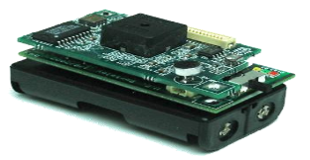
\includegraphics[width=7cm,height=3.7cm]{Chap1/1.png}
	\caption{Différence entre un optimum global et des optima locaux}
	\label{fig:CSF}
\end{figure}

\begin{algorithm}[H]
\SetAlgoLined
\KwResult{Write here the result }
 initialization\;
 \While{While condition}{
  instructions\;
  \eIf{condition}{
   instructions1\;
   instructions2\;
   }{
   instructions3\;
  }
 }
 \caption{How to write algorithms}
\end{algorithm}

	\item \textbf{Recherche tabou: } La méthode de recherche avec tabous, ou simplement recherche tabou (TS :Tabu Search) a été formalisée par Fred Glover en 1986 \cite{glover1986future} . Elle utilise explicitement l’historique de la recherche, à la fois pour échapper aux minimaux locaux et pour mettre en œuvre une stratégie d’exploration. Sa principale caractéristique est en effet basée sur  l’utilisation de mécanismes inspirés de la mémoire humaine. A l'inverse du recuit simulé qui génère de manière aléatoire une seule solution voisine s’ \( \in N(s) \) à chaque itération, la recherche tabou examine un échantillonnage de solutions de \( N(s) \) et retient la meilleure s’ même si s’ est plus mauvaise que s. La recherche tabou ne s'arrête donc pas au premier optimum trouvé. \\
	La méthode TS utilise une liste tabou, qui mémorise les dernières solutions rencontrées (ou des caractéristiques de solutions) vers lesquelles il est interdit de se déplacer. Ce procédé simple de mémoire permet de choisir le meilleur voisin non tabou, même si celui-ci dégrade la fonction-objectif f. Cependant, dans certains cas, les interdictions occasionnées par la liste tabou peuvent être jugées trop radicales. En effet, on risque d’éliminer (en les rendant tabous), certains mouvements particulièrement utiles. Pour éviter cela, on incorpore dans l’algorithme un mécanisme d’aspiration
qui détermine des critères selon lesquels un mouvement, bien que tabou, peut quand même être
accepté, s’il permet d’obtenir une meilleure solution que toutes celles déjà parcourues. \\
La taille de la liste tabou contrôle la mémoire du processus de recherche. Pour favoriser l’intensification, il suffit de diminuer la taille de la liste tabou. En revanche, augmenter la taille de la liste tabou, forcera le processus de recherche à explorer des régions plus vastes, favorisant ainsi la diversification. La taille de la liste tabou peut être modifiée au cours de la recherche \cite{battiti1994reactive} .\\
Une autre amélioration intéressante de la TS est l’utilisation de structure de mémoire à moyen et à long terme afin d’approfondir les notions d’intensification et de diversification.\\
\begin{figure}[h]
	\centering
	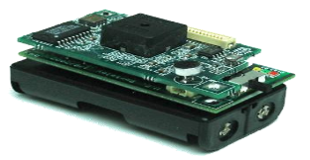
\includegraphics[width=7cm,height=3.7cm]{Chap1/1.png}
	\caption{Différence entre un optimum global et des optima locaux}
	\label{fig:CSF}
\end{figure}

\begin{algorithm}[H]
\SetAlgoLined
\KwResult{Write here the result }
 initialization\;
 \While{While condition}{
  instructions\;
  \eIf{condition}{
   instructions1\;
   instructions2\;
   }{
   instructions3\;
  }
 }
 \caption{How to write algorithms}
\end{algorithm}
	
	\item \textbf{Recherche locale : } Pour cette méthode de recherche il suffit de tester itérativement de nouvelles solutions potentielles dans la région de la solution courante, et de prendre la meilleure dans le voisinage. La méthode est une généralisation de la méthode de la descente de gradient elle consiste à partir d’une solution s à choisir une solution s’ dans un voisinage de s, noté N(s). La nouvelle solution choisie est meilleure que la précédente sous la fonction objective. Cela nous permet d’explorer l’espace des combinaisons  de proche en proche, en partant d’une combinaison initiale et en sélectionnant à chaque itération une combinaison voisine de la combinaison courante, obtenue en lui appliquant une transformation élémentaire jusqu’à la convergence à un optimum local. L’algorithme  décrivant le principe général de la recherche locale:
\begin{algorithm}[H]
\SetAlgoLined
\KwResult{Write here the result }
 initialization\;
 \While{While condition}{
  instructions\;
  \eIf{condition}{
   instructions1\;
   instructions2\;
   }{
   instructions3\;
  }
 }
 \caption{How to write algorithms}
\end{algorithm}
\end{enumerate}



